% Preamble
\documentclass[11pt,reqno,oneside,a4paper]{article}
\usepackage[a4paper,includeheadfoot,left=20mm,right=20mm,top=20mm,bottom=20mm]{geometry} %sets up the margins

%%%%%%%%%%%%%%%%%%%%%%%%%%%%%%%%%%%%%%%%%%%%%%%%%%%%%%%%%%%%%%%%%%%%%%%%%%%%%%%%
%
% This file contains some standard modifications to basic LaTeX2e and
% the article documentclass. Look through
% and make use of the shorthands defined herein.
%
%%%%%%%%%%%%%%%%%%%%%%%%%%%%%%%%%%%%%%%%%%%%%%%%%%%%%%%%%%%%%%%%%%%%%%%%%%%%%%%%

% Standard packages
\usepackage{amssymb,amsmath,amsthm}
\usepackage{xcolor,graphicx}
\usepackage{verbatim}
\usepackage{hyperref}
% Layout of headers & footers
\usepackage{titling}
\usepackage{fancyhdr}
\pagestyle{fancy} \lhead{{\theauthor}} \chead{} \rhead{} \lfoot{} \cfoot{\thepage} \rfoot{}

% Hyphenation
\hyphenation{non-zero}

% Instructor's email address
\newcommand{\InstEmail}{dave.smith@yale-nus.edu.sg}

%% Mathmode shortcuts
% Number sets
\newcommand{\NN}{\mathbb N}              % The set of naturals
\newcommand{\NNzero}{\NN^0}              % The set of naturals including zero
\newcommand{\NNone}{\NN}                 % The set of naturals excluding zero
\newcommand{\ZZ}{\mathbb Z}              % The set of integers
\newcommand{\QQ}{\mathbb Q}              % The set of rationals
\newcommand{\RR}{\mathbb R}              % The set of reals
\newcommand{\CC}{\mathbb C}              % The set of complex numbers
\newcommand{\KK}{\mathbb K}              % An arbitrary field
% Modern typesetting for the real and imaginary parts of a complex number
\renewcommand{\Re}{\operatorname*{Re}} \renewcommand{\Im}{\operatorname*{Im}}
% Upright d for derivatives
\newcommand{\D}{\ensuremath{\,\mathrm{d}}}
% Make epsilons look more different from the element symbol
\renewcommand{\epsilon}{\varepsilon}
% Always use slanted forms of \leq, \geq
\renewcommand{\geq}{\geqslant}
\renewcommand{\leq}{\leqslant}
% Shorthand for some relations
\newcommand{\po}{\preceq}
\newcommand{\rel}{{\mathcal R}} \newcommand{\rels}{\mathbin{\scriptstyle{\mathcal R}}}
% Shorthand for "if and only if" symbol
\newcommand{\Iff}{\ensuremath{\Leftrightarrow}}
% Make bold symbols for vectors
\providecommand{\BVec}[1]{\mathbf{#1}}
% Barred forms of \oplus and \otimes to represent the descents of these binary operators
\newcommand{\oplusbar}{\mathbin{\ooalign{$\hidewidth\overline{\oplus}\hidewidth$\cr$\phantom{\oplus}$}}} \newcommand{\otimesbar}{\mathbin{\ooalign{$\hidewidth\overline{\otimes}\hidewidth$\cr$\phantom{\otimes}$}}}
% Mathematical operators used in Proof
\DeclareMathOperator{\sgn}{sgn}          % The signum of a real number
\DeclareMathOperator{\power}{\mathcal{P}} % The power set of a set
\DeclareMathOperator{\Id}{Id}            % The identity function
\DeclareMathOperator{\Fun}{Fun}          % The set of functions from one set to another
\DeclareMathOperator{\Perm}{Perm}        % The set of permutations on a set
\DeclareMathOperator{\GCD}{GCD}          % The greatest common divisor of two integers
\newcommand{\abs}[1]{\left\lvert#1\right\rvert} % The absolute value of a real number or modulus of a complex number, with automatically scaling delimiters


%%%%%%%%%%
% Define extra macros here, if you need them.
%%%%%%%%%%






% Theorem definitions in the amsthm standard
\newtheorem{thm}{Theorem}
\newtheorem{lem}[thm]{Lemma}
\newtheorem{sublem}[thm]{Sublemma}
\newtheorem{prop}[thm]{Proposition}
\newtheorem{cor}[thm]{Corollary}
\newtheorem{conc}[thm]{Conclusion}
\newtheorem{conj}[thm]{Conjecture}
\theoremstyle{definition}
\newtheorem{defn}[thm]{Definition}
\newtheorem{cond}[thm]{Condition}
\newtheorem{asm}[thm]{Assumption}
\newtheorem{ntn}[thm]{Notation}
\newtheorem{prob}[thm]{Problem}
\theoremstyle{remark}
\newtheorem{rmk}[thm]{Remark}
\newtheorem{eg}[thm]{Example}
\newtheorem*{hint}{Hint}

% \usepackage{tikz}

\title{Student lectures}
\author{NAMES}

% Document
\begin{document} %\pagenumbering{gobble}

\maketitle
\thispagestyle{fancy}

This document will contain all the students' presentations.

\tableofcontents

\clearpage
\section{Sultan's lecture} \label{sec:Sultan}
Sultan's lecture goes in here.
% It all goes within a single section, so begin with a \subsection{...}, not a \section{...}
% Don't try to compile this file alone, instead compile GITREPO/master/student-lecture-all or GITREPO/master/student-lecture-sultan
% which input this file.
% You should not add the latex head to this file, just start writing as if you already have a \section{...} in the line above line 1.
% Do NOT write \end{document} at the end.


\clearpage
\section{Toto's lecture} \label{sec:Toto}
Toto's lecture goes in here.
% It all goes within a single section, so begin with a \subsection{...}, not a \section{...}
% Don't try to compile this file alone, instead compile GITREPO/master/student-lecture-all or GITREPO/master/student-lecture-toto
% which input this file.
% You should not add the latex head to this file, just start writing as if you already have a \section{...} in the line above line 1.
% Do NOT write \end{document} at the end.


\clearpage
\section{Dion's lecture} \label{sec:Dion}
\subsection{Inversion of Fourier Transforms}
For a function $f$, we are able to perform a Fourier Transform on it to convert to $F$, and find solutions to the equations involving $F$.
However, we ultimately want the solutions to the equations involving $f$, not to its Fourier Transform.
Therefore, this approach will be useless if we cannot guarantee that we can convert $F$ back to $f$.
The Convergence Theorem for Fourier Transforms provides us with the guarantee that performing an inverse Fourier Transform on $F$ will get us back exactly $f$, except at the jump discontinuities of $f$.

\begin{defn}[Fourier Transform] \label{FTdefn}
The Fourier Transform of function $f$, denoted $F$, is defined as
$$F(\mu) = \frac{1}{2\pi}\int_{-\infty}^{\infty}f(\xi)e^{-i\mu\xi}\mathrm{d}\xi.$$
\end{defn}

\begin{thm}[Convergence Theorem for Fourier Transforms] \label{FTthm}
Let $f(x), -\infty < x < \infty$ be a real or complex-valued function that is piecewise smooth over each finite interval. \pause Suppose that $\int_{-\infty}^{\infty}|f(x)|\mathrm{d}x$ is convergent, and $F(\mu)$ is the Fourier Transform of $f(x)$. \pause Then for each point $x$,
$$\lim_{M\rightarrow\infty}\int_{-M}^{M} F(\mu)e^{i\mu x}\mathrm{d}\mu = \frac{1}{2}f(x+0) + \frac{1}{2}f(x-0)$$
where $x+0$ is the right limit and $x-0$ is the left limit for each $x$.
\end{thm}

This theorem tells us that the inverse Fourier Transform converges to the original function $f$ for all $x$ at which $f$ is continuous, since in that case the left limit and right limit are equal. If $f$ has a jump discontinuity at point $x$, then the inverse Fourier Transform converges to the average of the left and right limits: $\frac{1}{2}f(x+0) + \frac{1}{2}f(x-0)$, of $f$ at that point instead.

The following example illustrates Theorem \ref{FTthm}. Suppose we are given a ``square wave" (Figure \ref{SquareWaveEg}),
$$f(x) = \begin{cases}
      \displaystyle 0 & \mbox{if }x < a \\
      1 & \mbox{if }a \leq x \leq b \\
      0 & \mbox{if }x > b.
   \end{cases}$$

\begin{figure}[h]
\centering
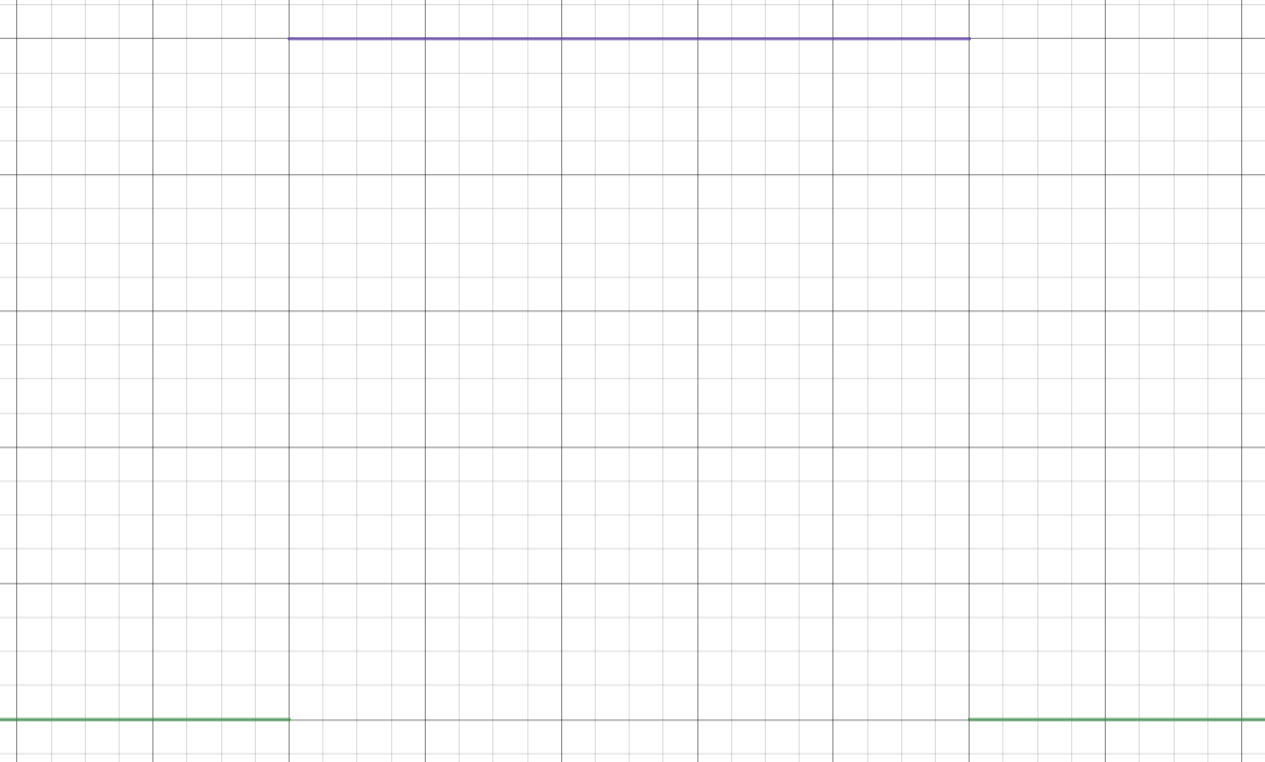
\includegraphics[scale=0.3]{Dion's_Images/SquareWaveEg.png}
\caption{Graph of the square wave}
\label{SquareWaveEg}
\end{figure}

If we find the Fourier Transform of the square wave and then inverse the Fourier Transform, we will get
$$\lim_{M\rightarrow\infty}\int_{-M}^{M} F(\mu)e^{i\mu x}\mathrm{d}\mu = \begin{cases}
      \displaystyle 0 & \mbox{if }x < a \\
      \textbf{0.5} & \textbf{\mbox{if }x = a} \\
      1 & \mbox{if }a < x < b \\
      \textbf{0.5} & \textbf{\mbox{if }x = b} \\
      0 & \mbox{if }x > b
   \end{cases}$$
   which is the original function except for at the jump discontinuities $x = a$ and $x = b$.
   See figure \ref{SquareWaveLimit} for an illustration of what happens at a jump discontinuity of the square wave.

\begin{figure}[h]
\centering
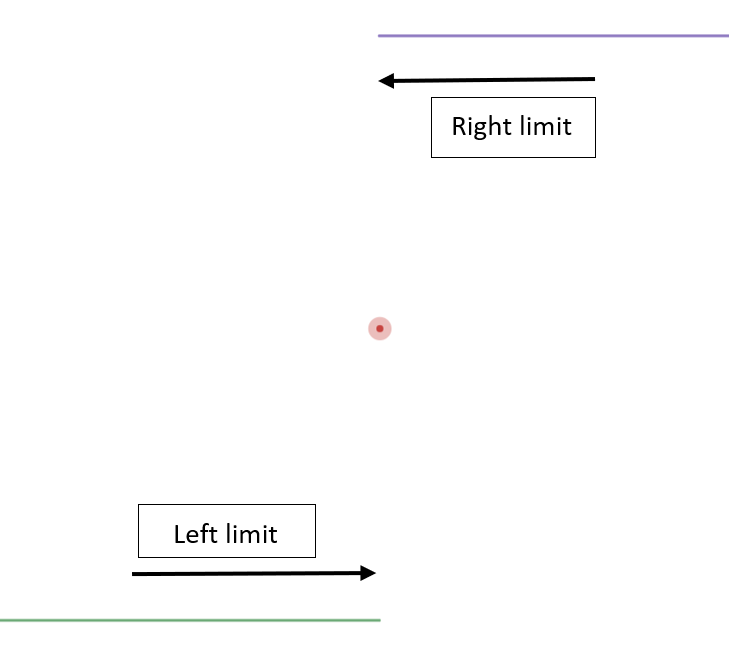
\includegraphics[scale=0.4]{Dion's_Images/SquareWave.png}
\caption{At jump discontinuities, the inverse Fourier Transform produces a point that is the average of the left and right limits of the original function at that point.}
\label{SquareWaveLimit}
\end{figure}

In order to prove the Convergence Theorem for Fourier Transforms (Theorem \ref{FTthm}) we will require Riemann's Lemma.

\subsection{Riemann's Lemma} \label{subsec:Riemann'sL}

\begin{lem}[Riemann's Lemma] \label{Riemann'sL}
If $f$ and $f'$ are piecewise continuous on $(a,b)$, then
$$ \lim_{\lambda\rightarrow\infty}\int_a^b f(x)sin(\lambda x) \mathrm{d}x = 0.$$
\end{lem}

Note that another way to say that $f$ and $f'$ are piecewise continuous on $(a,b)$ is to say that $f$ is \textbf{piecewise continuously differentiable}.
This is a weaker condition than \textbf{piecewise smooth} which means that $f$ and all of its derivatives are piecewise continuous.

Riemann's Lemma essentially states that as $\lambda\rightarrow\infty$,
the area of $f(x)\sin(\lambda x)$ above the $x$-axis and the area of $f(x)\sin(\lambda x)$ below the $x$-axis will cancel out completely.
\href{https://www.desmos.com/calculator/dxhg89t1te}{Click here for a graphical illustration of Riemann's Lemma.}

\begin{proof}
$$\int_a^b f(x)\sin(\lambda x) \mathrm{d}x = \sum_{i=0}^p\int_{x_i}^{x_i + 1} f(x)\sin(\lambda x) \mathrm{d}x$$
which is the sum of the continuous differentiable pieces of the function. See figure \ref{sumpieces} for an illustration of such a summation.

\begin{figure}[h]
\centering
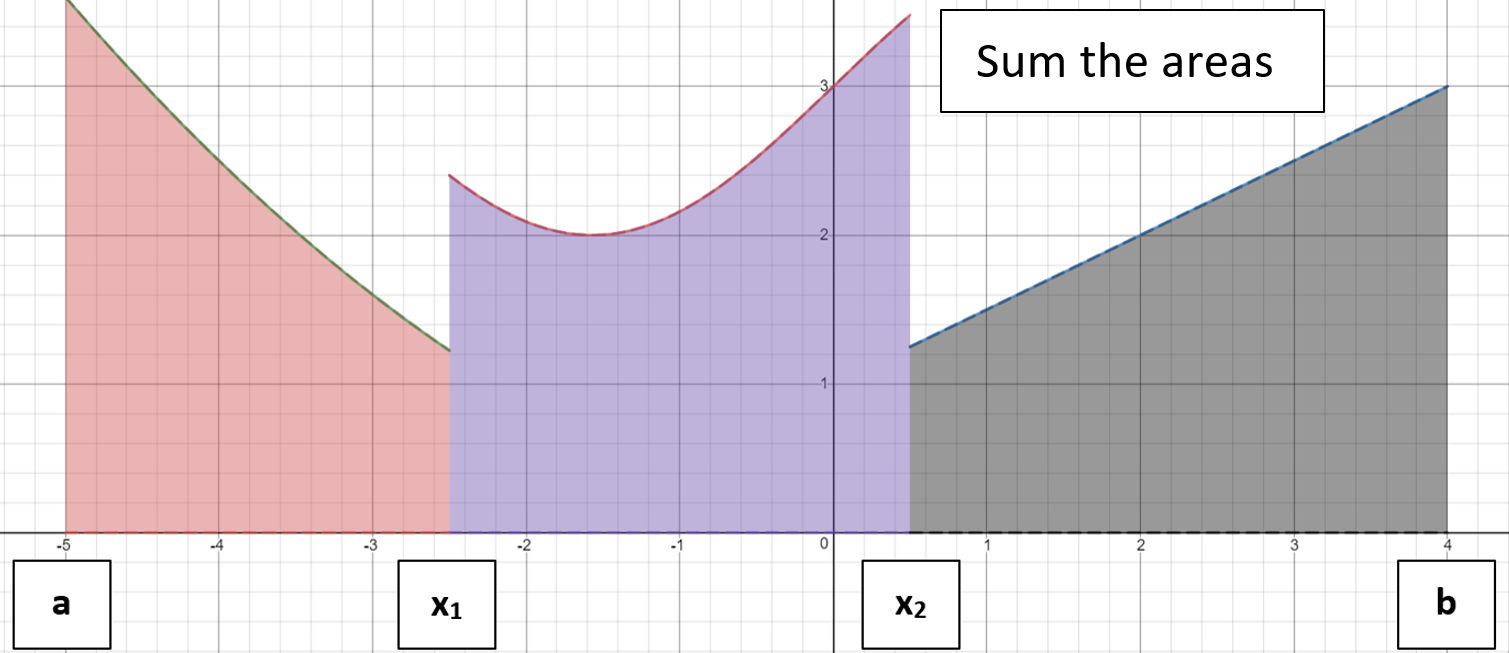
\includegraphics[scale=0.3]{Dion's_Images/Graph2.png}
\caption{The total area of a piecewise continuous differentiable function is the sum of the area of each of its continuous differentiable pieces.}
\label{sumpieces}
\end{figure}

We want to show that each continuous piece converges to $0$, i.e.
$$\lim_{\lambda\rightarrow\infty}\int_{x_i}^{x_{i + 1}} f(x)\sin(\lambda x) \mathrm{d}x = 0.$$
Perform integration by parts with $u = f(x)$ and $v' = \sin(\lambda x)$.
Note that since we are differentiating $f$ at this step, we require that $f$ be differentiable on $(x_i, x_{i + 1}})$.

Then,
$$\int_{x_i}^{x_{i + 1}} f(x)\sin(\lambda x) \mathrm{d}x = \left[ \frac{-f(x)\cos(\lambda x)}{\lambda} \right]_{x_i}^{x_{i+1}} + \frac{1}{\lambda}\int_{x_i}^{x_{i + 1}} f'(x)\cos(\lambda x) \mathrm{d}x.$$

If $\forall x_i \in [a,b], f(x_i)$ is finite, then
    $$\lim_{\lambda\rightarrow\infty}\left[ \frac{-f(x)\cos(\lambda x)}{\lambda} \right]_{x_i}^{x_{i+1}} = 0$$
since the numerator is always finite but the denominator grows to infinity. Moreover,
	$$\int_{x_i}^{x_{i + 1}}f'(x) \mathrm{d}x \geq \int_{x_i}^{x_{i + 1}} f'(x)\cos(\lambda x) \mathrm{d}x.$$
Therefore, $$\lim_{\lambda\rightarrow\infty}\frac{\left[ f(x)\right]_{x_i}^{x_{i+1}}}{\lambda} = 0 \implies \lim_{\lambda\rightarrow\infty}\frac{\int_{x_i}^{x_{i + 1}} f'(x)\cos(\lambda x) \mathrm{d}x}{\lambda} = 0.$$
Note that since this last step involves the integration of $f'$, it requires that $f'$ be continuous on $(x_i, x_{i + 1}})$.
\end{proof}

Now we are ready to prove the Convergence Theorem for Fourier Transforms (Theorem \ref{FTthm}).
\begin{proof}
$$2\pi\int_{-M}^{M}F(\mu)e^{i\mu x}\mathrm{d}\mu = \int_{-M}^{M}\left(\int_{-\infty}^{\infty}f(\xi)e^{-i\mu\xi}\mathrm{d}\xi\right) e^{i\mu x}\mathrm{d}\mu$$
by substitution of $F(\mu)$ (see Definition \ref{FTdefn}).
\begin{align}
\int_{-M}^{M}\left(\int_{-\infty}^{\infty}f(\xi)e^{-i\mu\xi}\mathrm{d}\xi\right) e^{i\mu x}\mathrm{d}\mu = \int_{-\infty}^{\infty}\left(\int_{-M}^{M}f(\xi)e^{-i\mu\xi}\mathrm{d}\mu \right) e^{i\mu x} \mathrm{d}\xi. \label{interchange}
\end{align}
The order of integration was switched. This requires a great deal of justification, but we will deal with it later in \S\ref{justification}. Proceeding, we have

\begin{align*}
    \int_{-\infty}^{\infty}\left(\int_{-M}^{M}f(\xi)e^{-i\mu\xi}\mathrm{d}\mu \right) e^{i\mu x} \mathrm{d}\xi &= \int_{-\infty}^{\infty}\left(\int_{-M}^{M}f(\xi)e^{i\mu(x-\xi)}\right)\mathrm{d}\mu \mathrm{d}\xi \\
    &= \int_{-\infty}^{\infty}\left[f(\xi)\frac{e^{i\mu(x-\xi)}}{i(x-\xi)}\right]_{-M}^{M}\mathrm{d}\xi \\
    &= \int_{-\infty}^{\infty}f(\xi)\left(\frac{e^{i M(x-\xi)} - e^{i(-M)(x-\xi)}}{i(x-\xi)}\right)\mathrm{d}\xi \\
    &= \int_{-\infty}^{\infty}f(\xi)\left(\frac{2i\sin(M(x-\xi))}{i(x-\xi)}\right)\mathrm{d}\xi \mbox{ (using a $\mathbb{C}$ identity)}\\
    &= 2\int_{-\infty}^{\infty}f(\xi)\left(\frac{\sin(M(x-\xi)}{x-\xi}\right)\mathrm{d}\xi.
\end{align*}
Substitute $\eta = \xi - x$ to get
$$2\int_{-\infty}^{\infty}f(x + \eta)\frac{\sin M \eta}{\eta}\mathrm{d}\eta = 2\int_{-\infty}^{\infty}\frac{f(x + \eta)}{\eta}\sin (M \eta)\mathrm{d}\eta.$$

However, what if $\eta = 0$? Do we get a division by zero? If $\eta = 0$, then $x = \xi$. This implies that 
$$\int_{-M}^{M}e^{i\mu(x-\xi)}\mathrm{d}\mu = \int_{-M}^{M}e^{i\mu(0)}\mathrm{d}\mu = \int_{-M}^{M}1\mathrm{d}\mu = 0.$$
Therefore, we can effectively ignore the case of $\eta = 0$ in the integration interval.

Using Riemann's Lemma (Lemma \ref{Riemann'sL}), for some $\delta \in \mathbb{C}$,
\begin{align*}
&\lim_{M\rightarrow\infty}\int_{\delta}^{\infty}\frac{f(x + \eta)}{\eta}\sin (M \eta)\mathrm{d}\eta = 0 \mbox{ and} \\
&\lim_{M\rightarrow\infty}\int_{-\infty}^{-\delta}\frac{f(x + \eta)}{\eta}\sin (M \eta)\mathrm{d}\eta = 0.
\end{align*} \pause
Therefore, we only have to analyse the integral for $-\delta \leq \eta \leq \delta$.

Riemann's Lemma (Lemma \ref{Riemann'sL}) also tells us that these two other integrals,
\begin{align*}
&2\int_{0}^{\delta}\frac{\sin M \eta}{\eta}(f(x + \eta) - f(x+0))\mathrm{d}\eta \hspace{1pc} \mbox{and}\\
&2\int_{-\delta}^{0}\frac{\sin M \eta}{\eta}(f(x + \eta) - f(x-0))\mathrm{d}\eta
\end{align*}
tend to $0$ as $M \rightarrow \infty$. We will use these two integrals to introduce the left and right limits to our proof.

Since
\begin{align*}
&2\lim_{M\rightarrow\infty} \int_{0}^{\delta}\frac{\sin M \eta}{\eta}(f(x + \eta) - f(x+0))\mathrm{d}\eta \\
&= \lim_{M\rightarrow\infty}\left( 2\int_{0}^{\delta}\frac{\sin M \eta}{\eta}f(x + \eta)\mathrm{d}\eta - 2\int_{0}^{\delta}\frac{\sin M \eta}{\eta} f(x+0)\mathrm{d}\eta\right)
\end{align*}
converges (to $0$)  and
$$2\int_{0}^{\delta}\frac{\sin M \eta}{\eta} f(x+0)\mathrm{d}\eta$$ converges, specifically to $\pi f(x+0)$ (see \href{https://en.wikipedia.org/wiki/Dirichlet_integral}{``Dirichlet Integral"} and \href{http://mathworld.wolfram.com/SincFunction.html}{``Sinc function"}),
we can split the limit into two terms, i.e.
\begin{align}
&2\lim_{M\rightarrow\infty} \int_{0}^{\delta}\frac{\sin M \eta}{\eta}(f(x + \eta) - f(x+0))\mathrm{d}\eta \nonumber \\
&= \lim_{M\rightarrow\infty}\left( 2\int_{0}^{\delta}\frac{\sin M \eta}{\eta}f(x + \eta)\mathrm{d}\eta\right) - \lim_{M\rightarrow\infty}\left(2\int_{0}^{\delta}\frac{\sin M \eta}{\eta} f(x+0)\mathrm{d}\eta\right) = 0 \nonumber \\
&= \lim_{M\rightarrow\infty}\left( 2\int_{0}^{\delta}\frac{\sin M \eta}{\eta}f(x + \eta)\mathrm{d}\eta\right) - \pi f(x+0) = 0. \label{limitR}
\end{align}
Similarly,
\begin{align}
&2\lim_{M\rightarrow\infty} \int_{-\delta}^{0}\frac{\sin M \eta}{\eta}(f(x + \eta) - f(x-0))\mathrm{d}\eta \nonumber \\
&= \lim_{M\rightarrow\infty}\left( 2\int_{-\delta}^{0}\frac{\sin M \eta}{\eta}f(x + \eta)\mathrm{d}\eta\right) - \lim_{M\rightarrow\infty}\left(2\int_{-\delta}^{0}\frac{\sin M \eta}{\eta} f(x-0)\mathrm{d}\eta\right) = 0 \nonumber \\
&= \lim_{M\rightarrow\infty}\left( 2\int_{-\delta}^{0}\frac{\sin M \eta}{\eta}f(x + \eta)\mathrm{d}\eta\right) - \pi f(x-0) = 0 \label{limitL}
\end{align}
since
$$2\lim_{M\rightarrow\infty}\int_{-\delta}^{0}\frac{\sin M \eta}{\eta} f(x-0)\mathrm{d}\eta = \pi f(x-0).$$
Note that the sinc function, $\frac{\sin \eta}{\eta}$, is symmetric about the $y$-axis (see figure \ref{sinc}).

\begin{figure}[h]
\centering
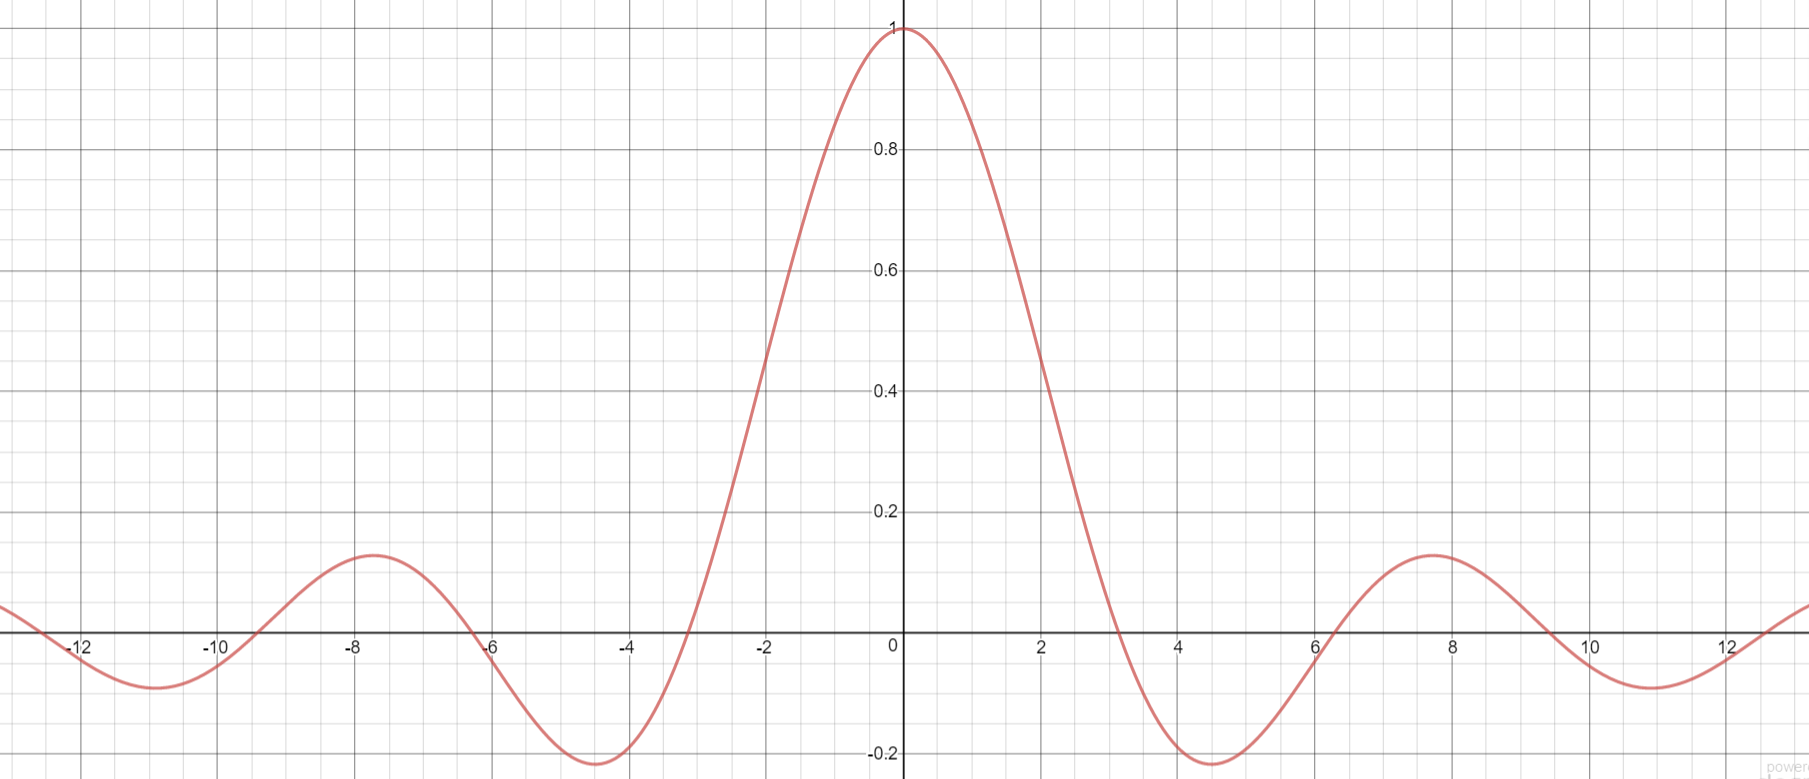
\includegraphics[scale=0.25]{Dion's_Images/sincgraph.png}
\caption{Graph of $\frac{\sin \eta}{\eta}$. The graph is symmetric about the $y$-axis.}
\label{sinc}
\end{figure}

Summing equations (\ref{limitR}) and (\ref{limitL}), we get
\begin{align*}
&2\lim_{M\rightarrow\infty} \int_{0}^{\delta}\frac{\sin M \eta}{\eta}(f(x + \eta) - f(x+0))\mathrm{d}\eta + 2\lim_{M\rightarrow\infty} \int_{-\delta}^{0}\frac{\sin M \eta}{\eta}(f(x + \eta) - f(x-0))\mathrm{d}\eta \\
&= 2\lim_{M\rightarrow\infty}\left(\int_{0}^{\delta}\frac{\sin M \eta}{\eta}f(x + \eta)\mathrm{d}\eta\right) - \pi f(x+0) + 2\lim_{M\rightarrow\infty}\left(\int_{-\delta}^{0}\frac{\sin M \eta}{\eta}f(x + \eta)\mathrm{d}\eta\right) - \pi f(x-0) = 0.
\end{align*}
This implies that
\begin{align*}
&2\pi\lim_{M\rightarrow\infty}\int_{-M}^{M}F(\mu)e^{i\mu x}\mathrm{d}\mu = 2\lim_{M\rightarrow\infty}\int_{-\delta}^{\delta}\frac{\sin M \eta}{\eta}f(x + \eta)\mathrm{d}\eta = \pi(f(x+0) + f(x-0)) \\
&\implies \lim_{M\rightarrow\infty}\int_{-M}^{M}F(\mu)e^{i\mu x}\mathrm{d}\mu = \frac{1}{2}(f(x+0) + f(x-0)) \mbox{ (divide both sides by $2\pi$)}.
\end{align*}
\end{proof}

\subsection{Justification for the Interchange of Integration Order} \label{justification}
Back during the step (\ref{interchange}), we interchanged the order of integration. For this step to be valid, we require that
$$\int_{-\infty}^{\infty}f(\xi)e^{-i\mu\xi}\mathrm{d}\xi$$ converges absolutely and converges uniformly.

We are given that
$$\int_\infty^{-\infty}|f(x)|\mathrm{d}x$$ 
is convergent. Therefore,
\begin{align*}
\left|\int_{-\infty}^{\infty}f(\xi)e^{-i\mu\xi}\mathrm{d}\xi\right| &= \int_{-\infty}^{\infty}|f(\xi)| |e^{-i\mu\xi}|\mathrm{d}\xi \\
&= \int_{-\infty}^{\infty}|f(\xi)| \mathrm{d}\xi \\
&= \int_{-\infty}^{\infty}|f(x+\eta)| \mathrm{d}x
\end{align*}
must also be convergent. This implies absolute convergence. Moreover, observe that 
$\left|\int_{-\infty}^{\infty}f(\xi)e^{-i\mu\xi}\mathrm{d}\xi\right|$ is independent of $\mu$, 
which implies that it converges uniformly.
This in turn implies that $\int_{-\infty}^{\infty}f(\xi)e^{-i\mu\xi}\mathrm{d}\xi$ converges uniformly (in fact, we say that the integral demonstrates \textbf{uniform absolute-convergence}).

For more information on the interchange of integration order, you may refer to \url{https://en.wikipedia.org/wiki/Order_of_integration_(calculus)}.

Now that we have proven the Convergence Theorem for Fourier Transforms (Theorem \ref{FTthm}), we can formally define the Inverse Fourier Transform.

\begin{defn}[Inverse Fourier Transform]
The Inverse Fourier Transform of function $F$ to get back $f$ is defined as
$$f(x) = \int_{-\infty}^{\infty}F(\mu)e^{i\mu x}\mathrm{d}\mu.$$
\end{defn}

\subsection{Calculus with Complex-valued Functions}
A complex-valued function is a function from any set $D$ to the set of complex numbers $\mathbb{C}$, i.e.
$$f:D\rightarrow\mathbb{C}.$$
In summary, almost every property of calculus with real-valued functions applies to calculus with complex-valued functions, with the notable exception of the mid-point theorems. Mid-point theorems do not work because we are now dealing with at least $3$-Dimensions.

An example of a midpoint theorem is Lagrange's Mean Value Theorem which states that: if $f$ is a continuous real valued function on $[a, b]$ which is
differentiable on $(a, b)$, then there exists $\xi \in (a, b)$ such that
$$f(b) - f(a) = f'(\xi)(b-a).$$
You can read more about the various midpoint (or mean value) theorems here: \url{https://en.wikipedia.org/wiki/Mean_value_theorem} (else you can take Real Analysis).

\subsection{Complex Differentiation}
\begin{defn}
Let $f$ be a complex-valued function defined on an open interval $(a,b)$. We define the
derivative of $f$ in the usual way by
$$f'(t) = \frac{\mathrm{d}}{\mathrm{d}t}f(t) = \lim_{h\rightarrow0}\frac{f(t+h) - f(t)}{h}.$$
\end{defn}
Note that
$$f'(t) = (\mbox{Re } f )'(t)+i (\mbox{Im }f )'(t),$$
and $f'(t)$ exists if and only if $(\mbox{Re }f )'(t)$ and $(\mbox{Im }f )'(t)$ both exist.
\medskip

\textbf{Properties of Complex Differentiation}
\begin{enumerate}
    \item $(\alpha f + \beta g)'(t) = \alpha f' (t) + \beta g' (t)$.
    \item $(fg)'(t) = f' (t) g (t) + f (t) g' (t)$ (Product rule).
    \item $(f \circ g)'(t) = f'(g(t))g'(t)$ (Chain rule).
\end{enumerate}

\subsection{Complex Integration}
\begin{defn}
Let $f$ be a piecewise continuous function defined on an interval
$[a,b]$ and taking values in the complex plane. We define the \textbf{Riemann} integral of $f$
as follows:
$$\int_a^b f(t) \mathrm{d}t = \int_a^b\mbox{Re }f(t)\mathrm{d}t + i \int_a^b\mbox{Im }f(t)\mathrm{d}t.$$
\end{defn}
As a direct consequence of this definition, we have
$$\mbox{Re }\int_a^b f(t) \mathrm{d}t = \int_a^b\mbox{Re }f(t)\mathrm{d}t \hspace{0.5pc} \mbox{and} \hspace{0.5pc} \mbox{Im }\int_a^b f(t) \mathrm{d}t = \int_a^b\mbox{Im }f(t)\mathrm{d}t$$

\medskip

\textbf{Properties of Complex Integration}
\begin{enumerate}
    \item $\displaystyle\int_a^b (f(t) \pm g(t)) \mathrm{d}t = \int_a^b f(t) \mathrm{d}t \pm \int_a^b g(t) \mathrm{d}t$.
    \item $\displaystyle\int_a^b \beta f(t) \mathrm{d}t = \beta\int_a^b f(t) \mathrm{d}t$.
    \item $\displaystyle\left|\int_a^b f(t) \mathrm{d}t\right| \leq \int_a^b |f(t)| \mathrm{d}t$ (Triangle Inequality for Integrals).
	\item If $c$ lies between $a$ and $b$ on the integration path, then $$\int_a^c f(t) \mathrm{d}t + \int_c^b f(t) \mathrm{d}t = \int_a^b f(t) \mathrm{d}t.$$
    \item If $f$ and $g$ are differentiable on $(a,b)$ and continuous on $[a,b]$, then integration by parts is valid, i.e. $$\int_a^b f(t)g'(t)\mathrm{d}t = \left[ f(t)g(t)\right]_a^b - \int_a^b f'(t)g(t)\mathrm{d}t.$$
\end{enumerate}

\begin{defn}[Antiderivative]
If $f$ is a piecewise continuous complex-valued function on $[a,b]$,
we say that $F$ is an antiderivative of $f$ if $F' = f$ at all the points of continuity of $f$ on $(a,b)$.
\end{defn}
This definition is based on the definition of differentiation.

\begin{thm}[Fundamental Theorem of Calculus]
Suppose that $f$ is a piecewise
continuous complex-valued function on the interval $[a, b]$ and let $F$ be a continuous antiderivative of $f$ in $[a, b]$. Then
$$\int_a^b f(t) \mathrm{d}t = F(b) - F(a).$$
\end{thm}
This theorem links the previously independent concepts of differentiation and integration.

\subsection{Parametrisation and Contour Integration}

\begin{defn}[Parametrisation]
A parametric form of a curve is a representation of the curve by a pair of equations $x = x(t)$ and $y = y(t)$, where $t$ ranges over a set of real numbers, usually a closed interval $[a,b]$. Each value of $t$ determines a point $\gamma(t) = (x(t),y(t)),$ which traces the curve as $t$ moves from $a$ to $b$.
\end{defn}

For example, we can parametrise a circle with equation $x^2 + y^2 = r^2$ as
$$ x = x(t) = r\cos(t),\hspace{1pc} y = y(t) = r\sin(t),\hspace{1pc} 0 \leq t \leq 2\pi, r \in \mathbb{R}.$$ \pause

A circle or circular arc has \textbf{positive orientation} if traversed in the counterclockwise orientation, and \textbf{negative orientation} if traversed in the clockwise direction. The circle defined above has positive orientation.

Parametrisation is especially useful when dealing with complex-valued functions.
Since $z = x+iy$, it makes sense to adopt the notation $$z(t) = x(t)+iy(t).$$ 
In particular, we can write the parametric form of a curve $\gamma$ using complex notation as $$\gamma(t) = x(t)+iy(t), a \leq t \leq b,$$ and think of the curve as the graph of a complex-valued function of a real variable $t$, i.e.
$$\gamma: \mathbb{R} \rightarrow \mathbb{C}.$$
In this way, we can go back to dealing with simpler and more familiar single variable real-valued functions.

\begin{defn}[Paths $\backslash$ Contours]
A path or a contour is a curve $\gamma$ defined on a closed interval $[a, b]$
which is continuously differentiable or piecewise continuously differentiable. The path $\gamma$ is called \textbf{closed} if $\gamma(a) = \gamma(b)$.
\end{definition}

\begin{defn}[Contour Integration]
Suppose that $\gamma$ is a path over a closed interval $[a, b]$ and that $f$ is a continuous complex-valued function defined
on the graph of $\gamma$. The path or contour integral of $f$ on $\gamma$ is defined as:
$$\int_\gamma f(z) \mathrm{d}z = \int_a^b f(\gamma(t))\gamma'(t) \mathrm{d}t$$
where $\gamma$ is parametrised in terms of $t$.
\end{defn}

Contour integration is akin to integration by substitution (with $z = \gamma(t), \mathrm{d}z = \gamma'(t)\mathrm{d}t$). See figure \ref{LineIntegral} for an illustration of contour integration.

\begin{figure}[h]
\centering
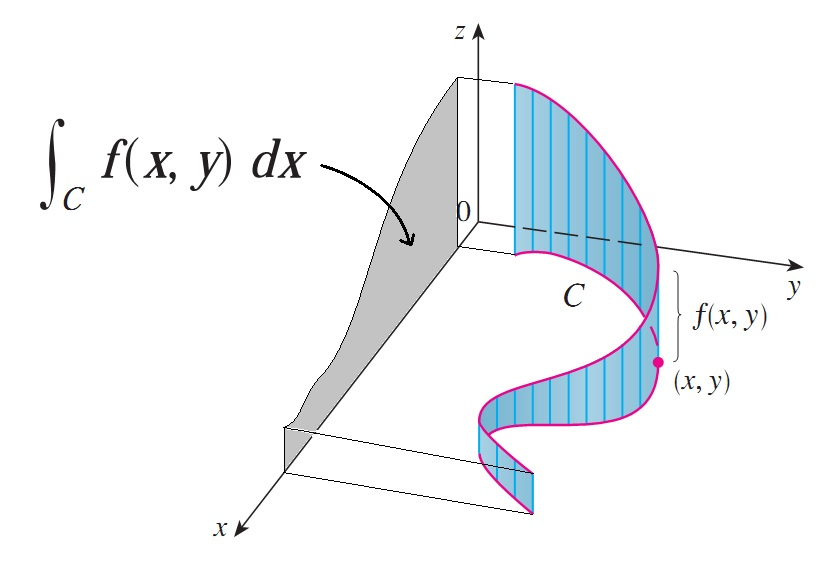
\includegraphics[scale=0.3]{Dion's_Images/LineIntegral.jpg}
\caption{An illustration of contour integration with the contour labeled as $C$. Image taken from \url{https://www.wikihow.com/Calculate-Line-Integrals}.}
\label{LineIntegral}
\end{figure}

\textbf{Properties of Contour Integration}
\begin{enumerate}
    \item $\displaystyle\int_\gamma (\alpha f(z) \pm \beta g(z)) \mathrm{d}z = \alpha\int_\gamma f(z) \mathrm{d}z \pm \beta\int_\gamma g(z) \mathrm{d}z$.
    \item Let $\gamma^*$ denote the reverse of $\gamma$ (for circular paths this means the reverse orientation), then $$\int_{\gamma^*} f(z) \mathrm{d}z = -\displaystyle\int_\gamma f(z) \mathrm{d}z.$$
    \item For $k = 1,\ldots,m$, let $\gamma_k$ be a path defined on $[k-1,k]$ such that $\gamma_k(k) = \gamma_{k+1}(k)$, for all $k \leq m-1$. If $f$ is a continuous function on the combined path $\Gamma = [\gamma_1,\gamma_2,\ldots, \gamma_m]$, then
    $$\int_\Gamma f(z) \mathrm{d}z = \sum_{k=1}^m \int_{\gamma_k} f(z) \mathrm{d}z.$$
\end{enumerate}

There are many different classes of parametrisations. We will only cover one specific class: polygonal paths.

\begin{defn}[Polygonal path]
A polygonal path $\gamma = [z_1, z_2, \ldots , z_n]$ is the
union of the line segments $[z_1, z_2], [z_2, z_3], \ldots, [z_{n-1}, z_n]$ for $z \in \mathbb{C}$. This is a piecewise linear path with initial point $z_1$ and terminal point $z_n$ and the path may have self intersections. \pause

A polygonal path is called \textbf{simple} if it does not have self intersections, except possibly at the endpoints, that is, $z_1$ and $z_n$ may coincide. The polygonal path is called \textbf{closed} if $z_1$ = $z_n$.
\end{defn}

Figures \ref{openppath} and \ref{closedppath} show some of the different types of polygonal paths. 
One notable use of polygonal paths is to approximate a more complicated contour, see figure \ref{approxcontour} for an example.

\begin{figure}[h]
\centering
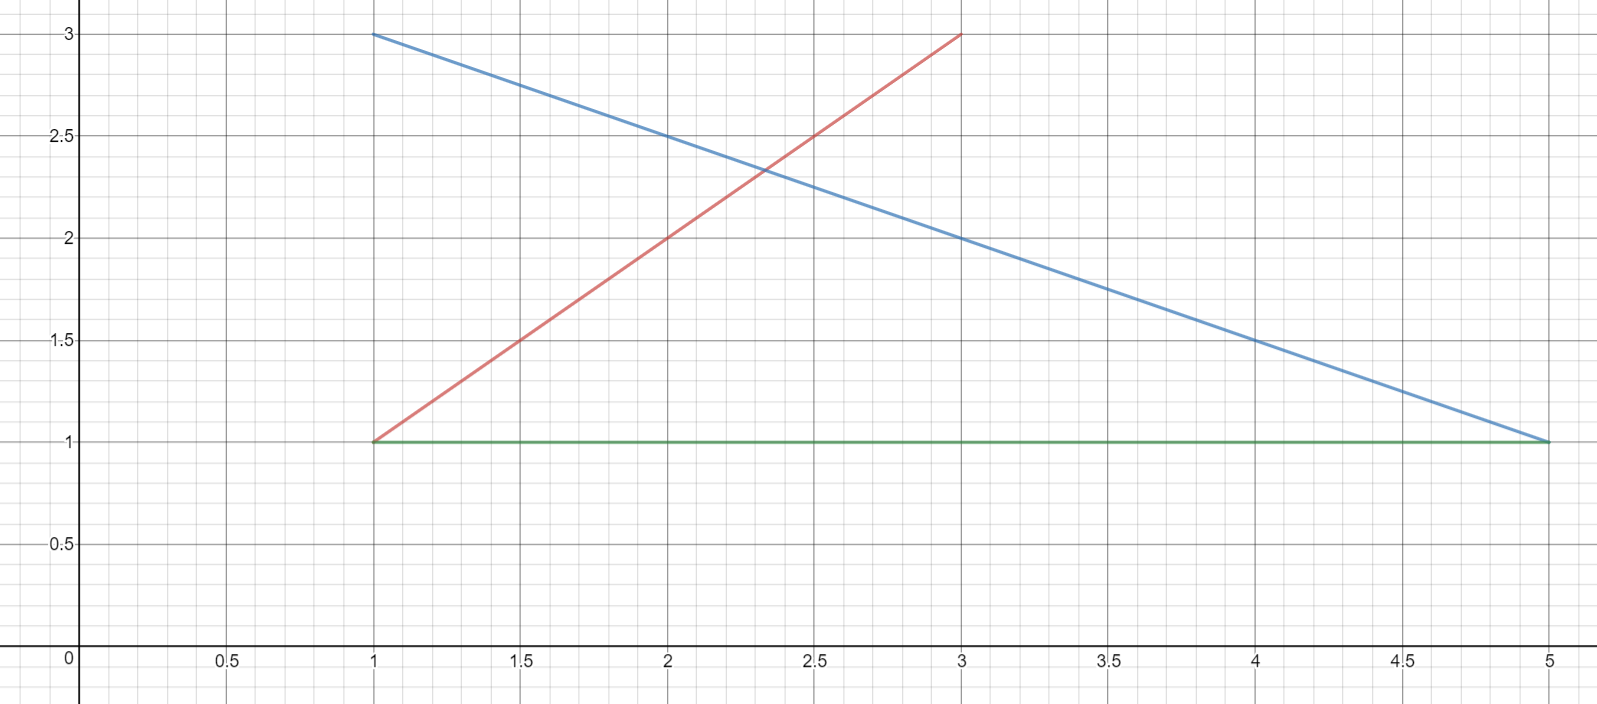
\includegraphics[scale=0.3]{Dion's_Images/OpenSIPolygonalPath.png}
\caption{This is a simple, closed, polygonal path.}
\label{openppath}
\end{figure}

\begin{figure}[h]
\centering
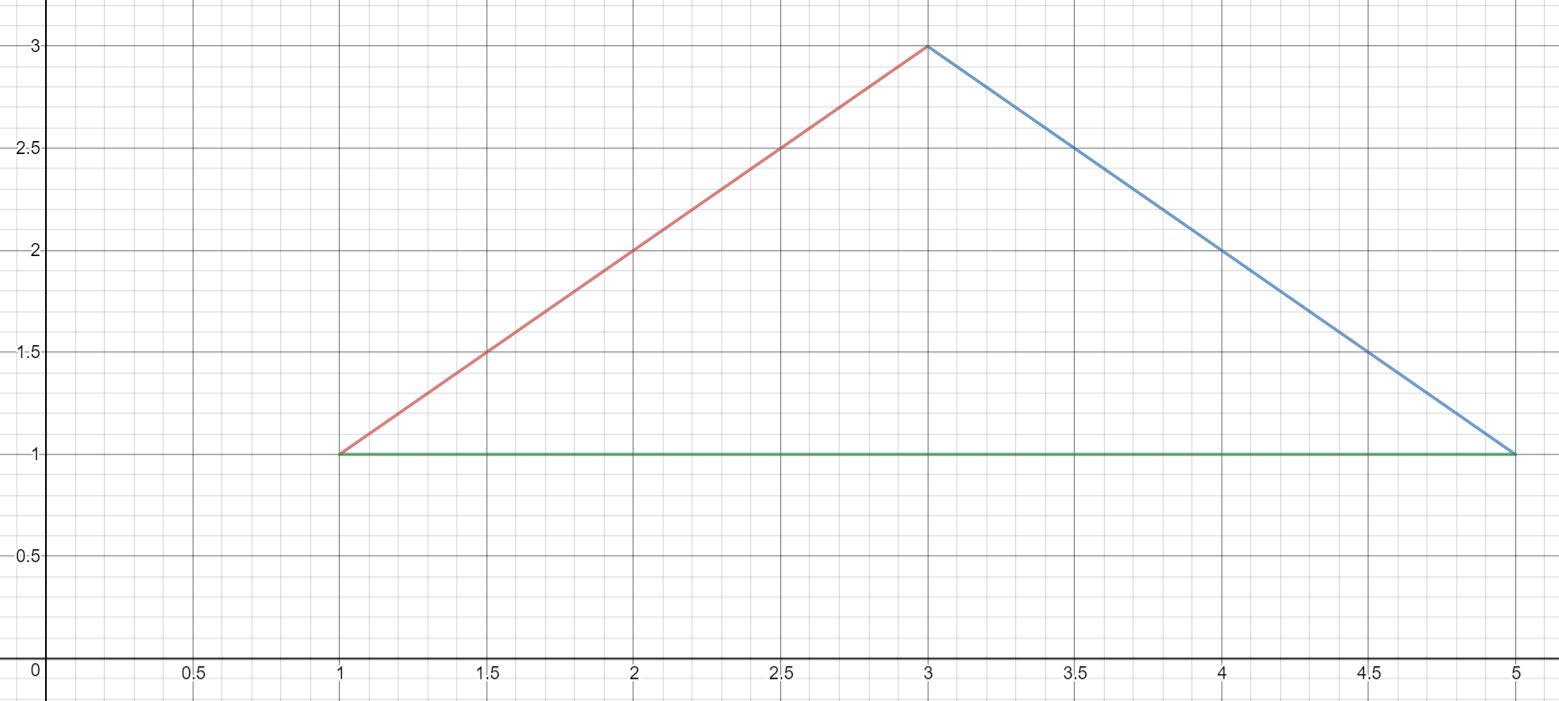
\includegraphics[scale=0.3]{Dion's_Images/ClosedPolygonalPath.png}
\caption{This is a self-intersecting, open, polygonal path.}
\label{closedppath}
\end{figure}

\begin{figure}[h]
\centering
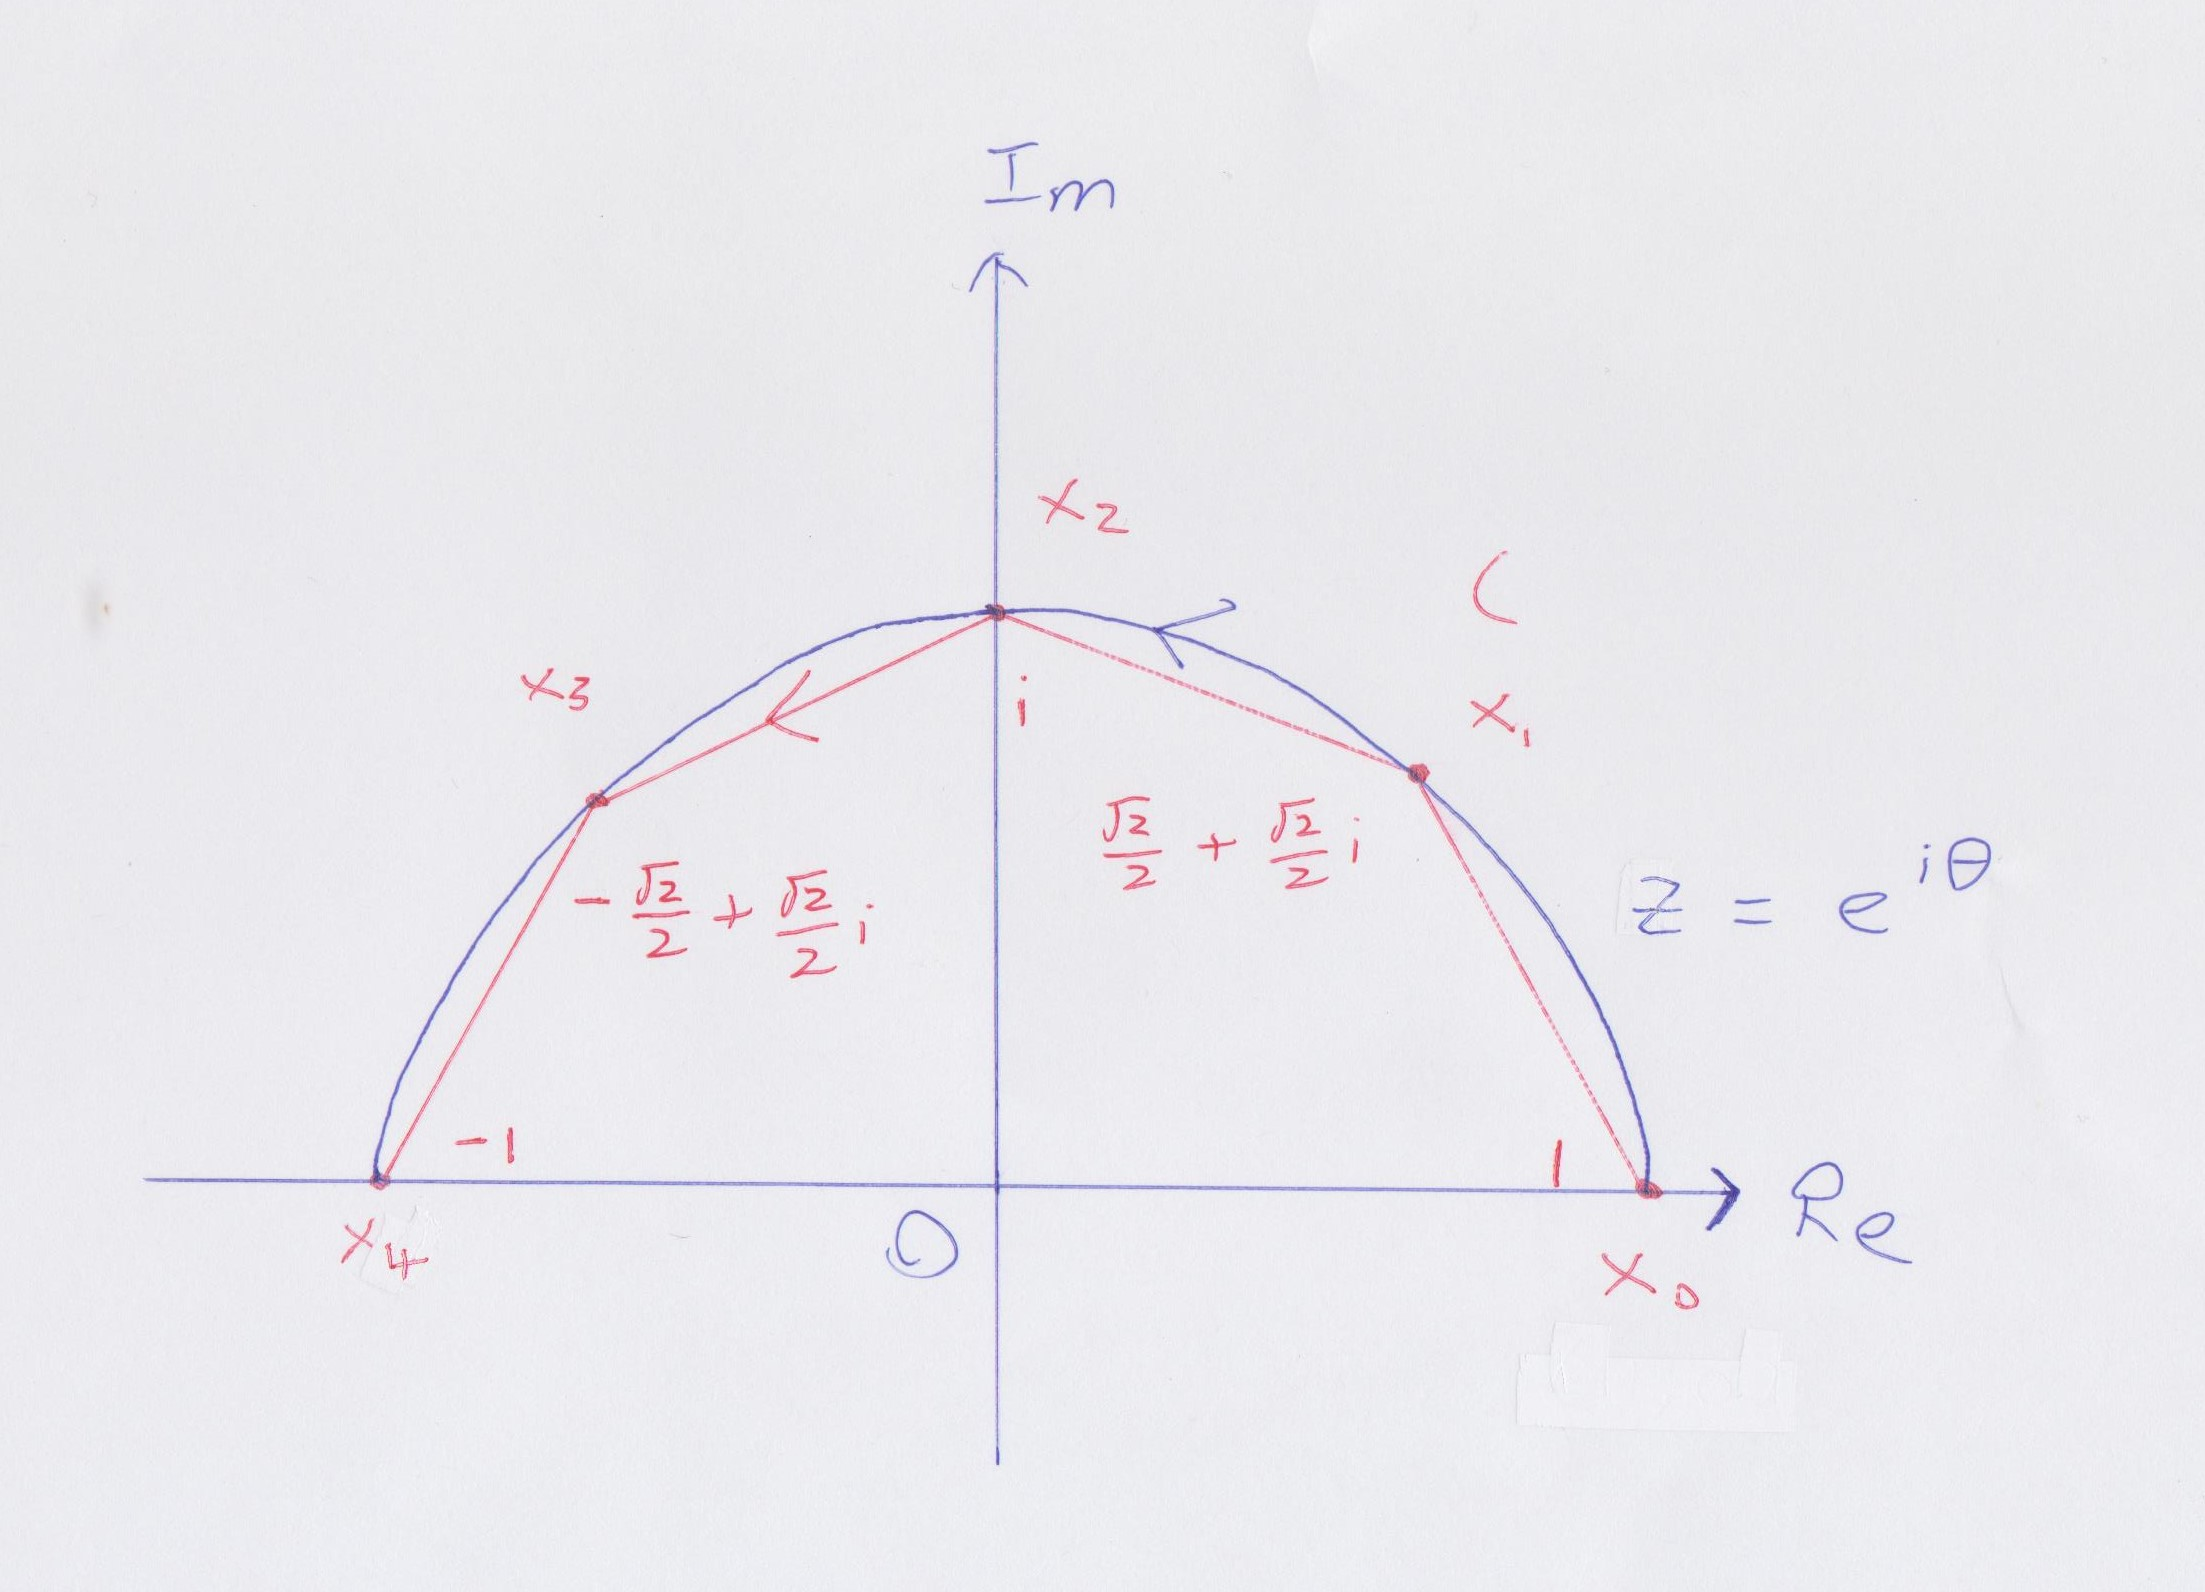
\includegraphics[scale=0.6]{Dion's_Images/ImprovedSemicircle.jpeg}
\caption{In this picture, a polygonal path is used to approximate a semicircle complex contour with positive orientation.}
\label{approxcontour}
\end{figure}

\subsection{Equivalent Parametrisations}
There are many different parametrisations, and they not unique to a function.
However, different parametrisations of the same function may be equivalent.

\begin{defn}[Equivalent Parametrisations]
We say that the paths $\gamma_1(t), a \leq t \leq b$, and $\gamma_2(s), c \leq s \leq d$, have equivalent parametrisations if there is a strictly increasing continuously differentiable function $\phi$ from $[c,d]$ onto $[a,b]$ such that $\phi(c) = a$ and $\phi(d) = b$ and $\gamma_2(s)=(\gamma_1 \circ \phi) (s)$ for all $s \in [c,d]$, or equivalently $\gamma_1(t)=(\gamma_2 \circ \phi^{-1})(t)$ for all $t \in [a,b]$, where $\phi^{-1}$ is the unique inverse of $\phi$.
\end{defn}
The term \textbf{strictly increasing} means that for any $s_1, s_2 \in [c,d]$, if $s_2 > s_1$, then $\phi(s_2) = t_2 > t_1 = \phi(s_1)$ for $t_1, t_2 \in [a,b]$.

\medskip
The following is a non-comprehensive list of rules regarding equivalent parametrisations:
\begin{enumerate}
\item If two paths do not have the same range, they are not equivalent.
\item For two paths $\gamma_1$ with endpoints $a,b$, and $\gamma_2$ with endpoints $c,d$, if $\gamma_1(a) \neq \gamma_2(c)$ or $\gamma_1(b) \neq \gamma_2(d)$, then the two paths are not equivalent.
\item If the trajectories of two paths are not the same, then they are not equivalent. This is a corollary of rule $2$. 
Though one can reverse the orientation of one path and recheck for equivalence.
\item For contours in the $xy$-plane, if two paths do not have the same number of turning points (both with respect to the $x$-axis, and w.r.t the $y$-axis), then they are not equivalent. 
Note that stationary points (derivative $= 0$) are not necessarily turning points.
\item Open paths are not equivalent to closed paths. This is a corollary of rule $2$.
\item If two paths are equivalent, then a bijection exists between their domains. 
That bijection is in fact the function $\phi$, which is why $\phi^{-1}$ exists.
\end{enumerate}

\begin{figure}[h]
\centering
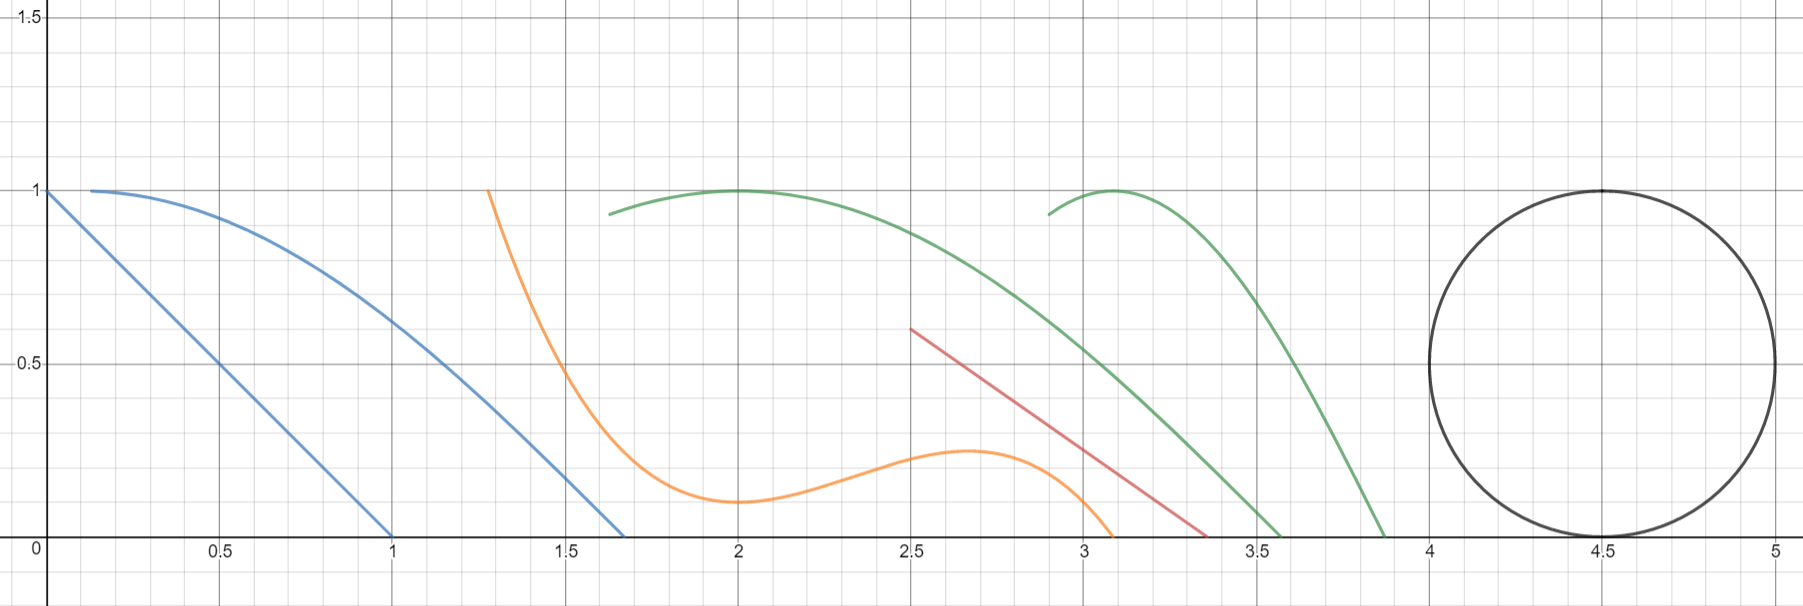
\includegraphics[width = \linewidth]{Dion's_Images/EquivalentPaths.png}
\caption{The paths in this picture have equivalent parametrisations if and only if they have the same colour. Assume the trajectories of the paths all have a left to right orientation. 
The graphs can be accessed here: \url{https://www.desmos.com/calculator/aaswr1xwcg}.}
\label{EquivalentPaths}
\end{figure}

In figure \ref{EquivalentPaths}, the red line is not equivalent to any other paths because its range is different from theirs.
The black circle is not equivalent to any other paths because it is a closed path whereas all the other paths are open. Also, it is the only path with turning points with respect to the $y$-axis.
The green and blue paths are not equivalent because of the endpoint rule (rule $2$).
Less evident is the fact that the orange path is not equivalent to the blue paths. This we will prove.
\begin{proof}
Suppose that the orange path, $\gamma_2$, and a blue path, $\gamma_1$, are equivalent.
Choose a point a small distance to the left of the leftmost turning point of the orange path. Denote this point $(c_1, \gamma_2(c_1))$. Then, there exists $\phi(c_1) = t_1$ such that $\gamma_1(t_1) = \gamma_2(c_1)$.
Since there is a turning point to the right of $(c_1, \gamma_2(c_1))$, there also exists $c_2$ such that $\gamma_2(c_2) = \gamma_1(t_1)$.
Then, $\phi^{-1}(t_1) = c_1$ and $\phi^{-1}(t_1) = c_2$. Since $\phi$ is bijective, this implies that $c_1 = c_2$. However, $c_1 < c_2$, which is a contradiction.
\end{proof}

Equivalent parametrisations are extremely important because of the following theorem:
\begin{thm}[Independence of Parametrisation]
Suppose that the paths $\gamma_1(t), a \leq t \leq b,$ and $\gamma_2(s), c \leq s \leq d$, have equivalent parametrisations and let $f$ be a continuous function on this path. Then
$$\int_{\gamma_1} f(z) \mathrm{d}z = \int_{\gamma_2} f(z) \mathrm{d}z.$$
\end{thm}
In one sentence, this theorem tells us that integrals over equivalent parametrisations produce identical results.
This theorem accords us with a great deal of flexibility when choosing parametrisations.

\begin{proof}
We have $\gamma_2 = \gamma_1 \circ \phi$ , where $\phi$ is a strictly increasing continuously differentiable function from $[c,d]$ onto $[a,b]$. Assume first that $\gamma_1$ is differentiable at every point on $(a,b)$. Then $\gamma_2 =\gamma_1 \circ \phi$ is also differentiable at every point on $(c,d)$.
Using $\gamma_2(s) =\gamma_1(\phi (s))$ and $\gamma'_2(s) = \gamma'_1(\phi(s))\phi'(s)$, we perform a change of variable with $t = \phi(s)$, $\mathrm{d}t = \phi'(s)\mathrm{d}s$, and obtain 
\begin{align*}
\int_c^d f(\gamma_2(s))\gamma'_2(s)\mathrm{d}s &= \int_c^d f(\gamma_1(\phi(s)))\gamma'_1(\phi(s))\phi'(s)\mathrm{d}s \\ 
&= \int_a^b f(\gamma_1(t))\gamma'_1(t)\mathrm{d}t.
\end{align*}
Therefore, parametrising with $z = \gamma_1(t)$ or $z = \gamma_2(s)$ produces equal integrals.
The same result will be obtained if the change of variable was performed with $s = \phi^{-1}(t)$ instead.
It remains to consider the case where $\gamma_1$ is not differentiable at some points $a_1 < \ldots < a_{m-1}$ in $(a,b)$.  Set $a_0 =a$ and $a_m =b$. Then $\gamma_1$ is differentiable at every point in the interval $(a_j,a_{j+1})$ for $j = 0,\ldots,m-1$.  The first part of our proof tells us that
$$\int_{\phi^{-1}(a_j)}^{\phi^{-1}(a_{j+1})} f(\gamma_2(s))\gamma'_2(s)\mathrm{d}s = \int_{a_j}^{a_{j+1}} f(\gamma_1(t))\gamma'_1(t)\mathrm{d}t.$$ 
Sum the integrals over $0 \leq j \leq m-1$. Since $c = \phi^{-1}(a_0) = \phi^{-1}(a)$ and $d = \phi^{-1}(a_m) = \phi^{-1}(b)$, we get
\begin{align*}
\int_c^d f(\gamma_2(s))\gamma'_2(s)\mathrm{d}s &= \int_{\phi^{-1}(a)}^{\phi^{-1}(b)} f(\gamma_2(s))\gamma'_2(s)\mathrm{d}s \\ 
&= \int_a^b f(\gamma_1(t))\gamma'_1(t)\mathrm{d}t.
\end{align*}
\end{proof}
% It all goes within a single section, so begin with a \subsection{...}, not a \section{...}
% Don't try to compile this file alone, instead compile GITREPO/master/student-lecture-all or GITREPO/master/student-lecture-dion
% which input this file.
% You should not add the latex head to this file, just start writing as if you already have a \section{...} in the line above line 1.
% Do NOT write \end{document} at the end.


\clearpage
\section{Xinyu's lecture} \label{sec:Xinyu}
Xinyu's lecture goes in here.
% It all goes within a single section, so begin with a \subsection{...}, not a \section{...}
% Don't try to compile this file alone, instead compile GITREPO/master/student-lecture-all or GITREPO/master/student-lecture-xinyu
% which input this file.
% You should not add the latex head to this file, just start writing as if you already have a \section{...} in the line above line 1.
% Do NOT write \end{document} at the end.



\end{document}


